\section{Simulation Results}%
\label{sec:simulations}

The simulation section illustrates the results in the order of detection, estimation and joint detection and estimation.
Four different lengths of reference symbol sequences are simulated with $50\%$ rolloff Square-Root Raised Cosine (SRRC) pulses.
The reference sample sequence is chosen from Gold sequence and modulated by a QPSK alphabet with good autocorrelation properties.
We assume the normalized frequency offset is small enough so that the design parameter $k$ of the SD estimator
can be chosen optimally by $2/3$ length of the preamble (For $K-$SD estimator, all the estimates of SD satisfying the aliasing limits). 
% may give more sentence here.

\subsection{Simulation Results for Detection}

\begin{figure}[t]
    \centerline{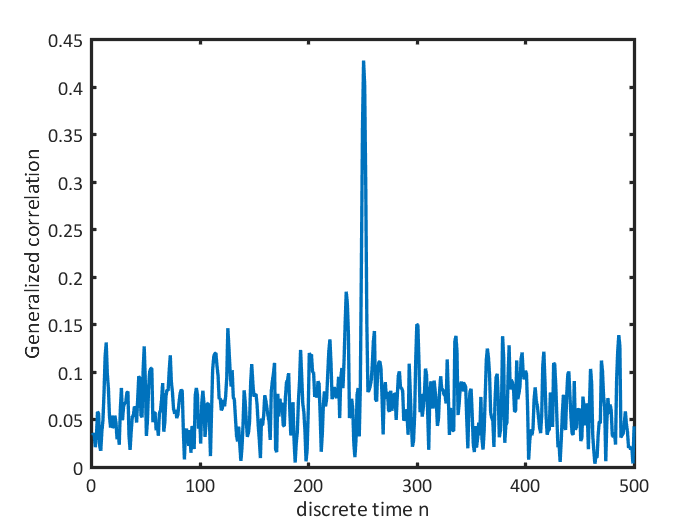
\includegraphics[width=3.4in]{generalized_correlation.png}}
    \caption{Performance of GLRT based detector of~\eqref{eq:generalized_corr} via the received stream}
    \label{fig:Generalized correlation}
    \end{figure}

\begin{figure}[t]
    \centerline{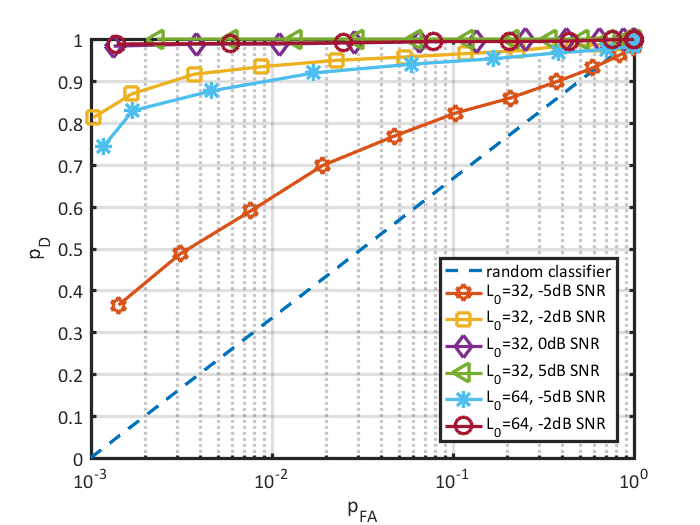
\includegraphics[width=3.4in]{receiver_operating_characteristics.png}}
    \caption{Receiver operating characteristics of detector for different SNR}
    \label{fig:Receiver operating characteristics}
    \end{figure}

\begin{figure}[t]
    \centerline{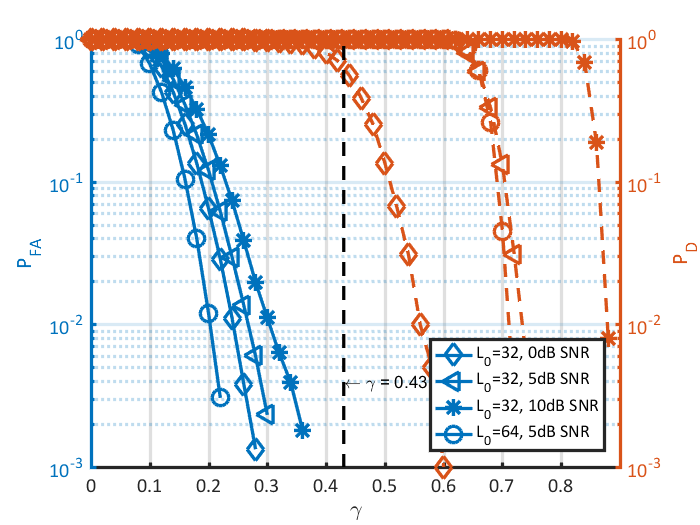
\includegraphics[width=3.4in]{false_alarm_and_detection_probability.png}}
    \caption{False alarm and detection ratio for different SNR and size of preamble}
    \label{fig:False alarm and detection}
    \end{figure}

Figure~\ref{fig:Generalized correlation} illustrates the performance of the proposed detector of~\eqref{eq:generalized_corr}. 
We see from the figure that it does not show a perfect autocorrelation property after pulse shaping, e.g., around the position of the preamble, 
the correlation decays very slow. The problem happens that it makes~\eqref{eq:generalized_corr} much more challengable to choose the threshold to 
distinguish between the real position of the preamble and its corresponding adjacent positions. The solution to mitigating it is to 
adjust the detection algorithm by changing making the decisions at each observation individually (by comparing the correlation and threshold) to
finding the local maximum of the correlation.

Figure~\ref{fig:Receiver operating characteristics} shows the receiver operating characteristics (ROC) of the proposed (adjusted) detector.
It basically illustrates that the detector has good ROCs at moderate SNR. Specifically, the detector achieves perfect ROCs for positive SNR (in decibel); 
Moreover, it is robust to low SNR environment, e.g., we can pick such a threshold to achieve 
$10^{-3}$ false alarm probability and $0.75$ detection probability simultaneously.
However, it is not clear from this figure to pick an exact threshold for certain detection purpose.

Figure~\ref{fig:False alarm and detection} shows the performance of detector but from another perspective. Specifically, it gives us a clearer insight into
the false alarm and detection probabilities via the threshold.
It is common that it's hard to pick such a threshold to accommodate all specific detection purposes.
For simulation purpose, if we want to determine a threshold to work for the reference signal sequence with $L_0 {\geq} 32$ and up to~\numb{10}\dB~SNR,
Based on Figure~\ref{fig:False alarm and detection} and Neyman-Pearson criterion, $\gamma=0.43$ is a good choice to meet $P_{\text{FA}}<1e^{-3}$ and nearly perfect $P_{\text{D}}$.

\subsection{Simulation Results for Estimation}

\begin{figure}[t]
    \centerline{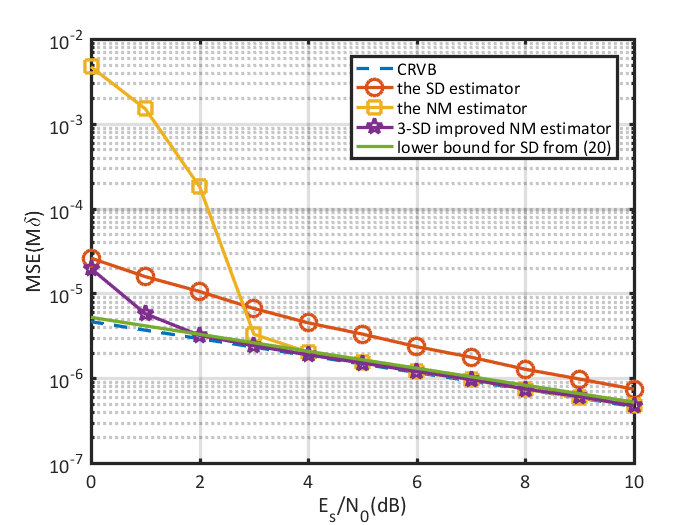
\includegraphics[width=3.4in]{accuracy_NM_SD.png}}
    \caption{Accuracy of the SD and SD (or $K$-SD) based NM estimators ($L_0=32$)}
    \label{fig:accuracy_NM_SD}
    \end{figure}

\begin{figure}[t]
    \centerline{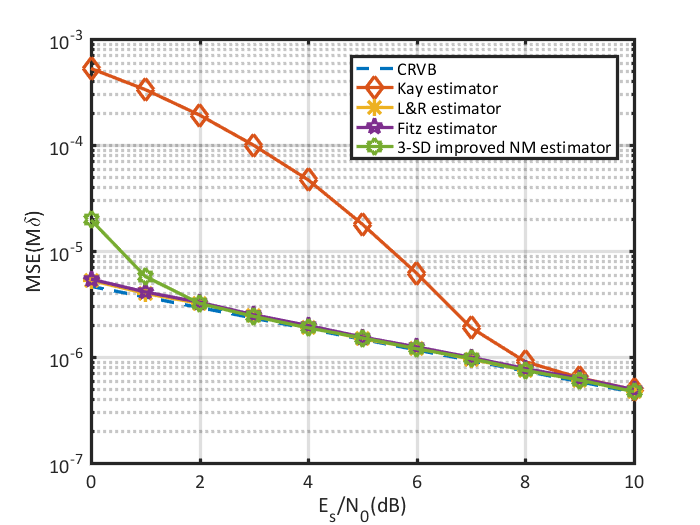
\includegraphics[width=3.4in]{accuracy_NM_traditional.png}}
    \caption{Accuracy of the NM and traditional estimators ($L_0=32$)}
    \label{fig:accuracy_NM_traditional}
    \end{figure}

\begin{figure}[t]
    \centerline{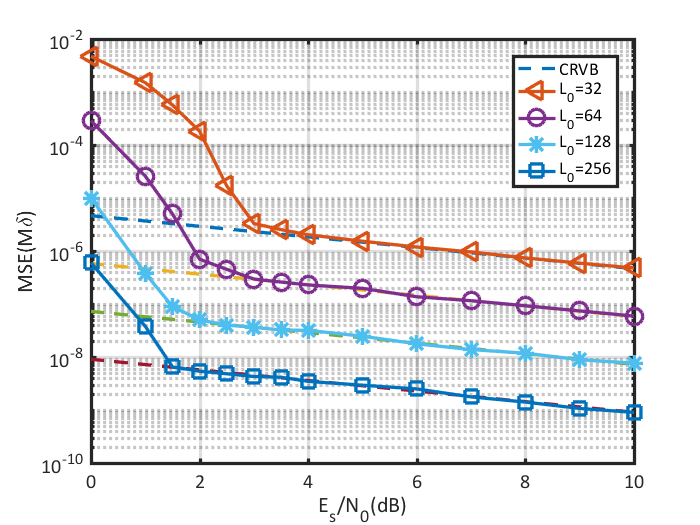
\includegraphics[width=3.4in]{freq_NM_with_different_size.png}}
    \caption{Accuracy of NM frequency estimate in joint detection and estimation ($\gamma=0.43$)}
    \label{fig:accuracy_freq_NM_joint}
    \end{figure}

\begin{figure}[t]
    \centerline{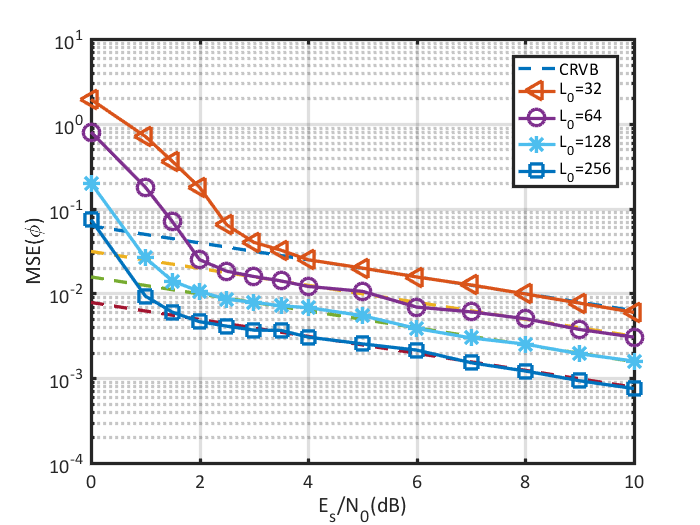
\includegraphics[width=3.4in]{phi_NM_with_different_size.png}}
    \caption{Accuracy of the NM phase estimate in joint detection and estimation ($\gamma=0.43$)}
    \label{fig:accuracy_phi_NM_joint}
    \end{figure}

\begin{figure*}[t]
    \centerline{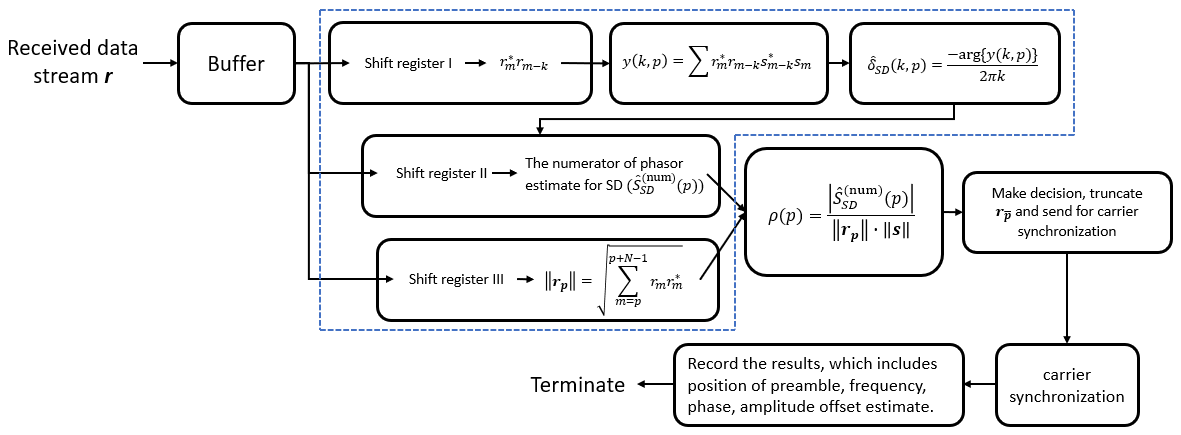
\includegraphics[width=6.5in]{SDR_receiver.png}}
    \caption{Block diagram for implementing the proposed algorithm on software-defined radio (some steps are omitted)}
    \label{fig:SDR_receiver}
    \end{figure*}

For simulation purpose, we assume that the detection pro\-gress is perfect in this section.
Figure~\ref{fig:accuracy_NM_SD} emphasizes illustrating the accuracy of the two proposed estimators, 
the SD estimator of~\eqref{eq:delta_SD} and the NM estimator of~\eqref{eq:iter_NM_est} in this paper.
The lower dashed line denotes the Cramer-Rao vector bound (CRVB) for frequency estimate, which is given by

\begin{equation}
    \label{eq:CRVB_freql}
    \text{CRVB}(M\delta) \geq \frac{3}{2\pi^{2}L_{0}^3E_s/N_{0}}.
  \end{equation}
Furthermore, the CRVB for $\phi$ is derived as

\begin{equation}
    \label{eq:CRVB_phi}
    \text{CRVB}(\phi) \geq \frac{2}{L_{0}E_s/N_{0}}.
  \end{equation}
The derivations of~\eqref{eq:CRVB_freql} and~\eqref{eq:CRVB_phi} are given in Appendix~\ref{BL}.

In Figure~\ref{fig:accuracy_NM_SD}, we see the NM estimator approaches the CRVB. The accuracy of the SD estimator is crucial
not only just for building the GLRT detector but deciding the accuracy of the NM estimator.
The evidence is that the NM estimator performs even worse than the SD estimator at low SNR.
This is because the Newton iteration of~\eqref{eq:iter_NM_est} converges occasionally to local
minimum away from the true frequency offset if the beginning estimate is really far from. Figure~\ref{fig:accuracy_NM_SD} also shows the averaging method of~\eqref{eq:K_SD_est}
improves the accuracy of the SD estimator thus improves the NM estimator at low SNR.

Figure~\ref{fig:accuracy_NM_traditional} compares the performance of the NM and traditional estimators in ~\cite{Kay_89,Luise_Reggiannini_95,Fitz_94}.
Related to Figure~\ref{fig:accuracy_NM_SD}, we conclude that the NM estimator can achieve as good accuracy as those autocorrelation-based estimators 
(L\&R estimator~\cite{Luise_Reggiannini_95} and Fitz estimator~\cite{Fitz_94})
when the SD estimator is accurate enough. To put it another way, without increasing complexity by averaging with multiple SD estimators, 
the NM estimator can achieve the same good accuracy as the traditional estimators at moderate SNR.

\subsection{Simulation Results for Detection and Synchronization}

This section simulates the complete signal acquisition chain and shows the simulation results of the last step in Figure~\ref{fig:sig_acquis_chain}.
Figure~\ref{fig:accuracy_freq_NM_joint} and~\ref{fig:accuracy_phi_NM_joint} illustrate the performance of our proposed joint detection and 
carrier synchronization algorithm. No averaged SD estimator is used because we want to reduce the complexity of the sequential detection process.
Compared with Figure~\ref{fig:False alarm and detection} and Figure~\ref{fig:accuracy_NM_SD}, the reason for the NM estimator not approaching the CRVB at low SNR
is due to the non-sufficient accuracy of the SD estimator. 
Besides that, we can also get a common result that by increasing
the size of the preamble, better performance of carrier synchronization is realized and CRVB is approached at lower SNR.
